\section{Проектирование мощного выходного каскада усилителя}

На четвертом этапе проектирования 
проводится расчет мощного выходного каскада (ВК)
на дискретных компонентах, необходимого для
расширения возможностей усилителя переменного тока
по выходной мощности и максимальному току нагрузки.

Рекомендуемая схема (ВК) представлена 
на рис.~\ref{fig:recommendedsheme}. 
На этом же рисунке приведена часть схемы усилителя,
приведенного на рис.~\ref{fig:sub2_py}
$ (DA_2; R_4; R_5; С_2) $, к выходу которого
подключен вход ВК.

\begin{figure}[H]
	\centering
	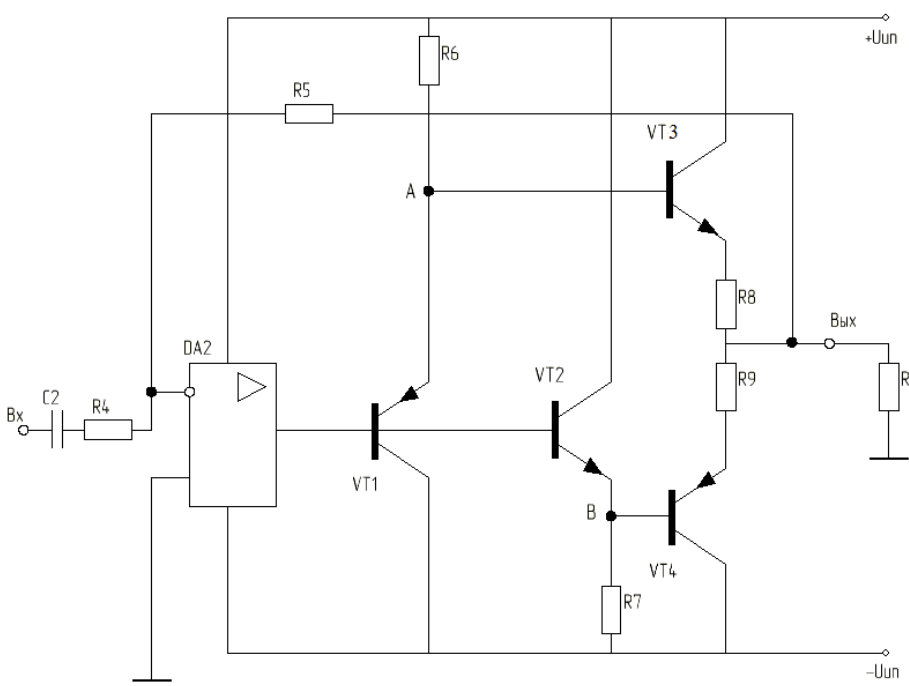
\includegraphics[width=0.7\linewidth]{photo/recommended_sheme}
	\caption{Рекомендуемая схема мощного выходного каскада}
	\label{fig:recommendedsheme}
\end{figure}

\subsection{Назначение и функционирование входного каскада}

Этот каскад $ (VT1 – VT4; R_6 – R_9) $
предназначен для получения большого 
тока нагрузки: $ I_н = 1 - 1,5~А) $.
Интегральный операционный усилитель $ DA2 $ серии 741
имеет максимальный ток нагрузки: $ I_н = 10 - 20~мА $,
что явно недостаточно для нашего усилителя.

Входной каскад усиливает только по току.
По напряжению его коэффициент передачи
близок к 1 (повторитель напряжения).
Действительно, транзисторы $ VT1 $  и $ VT3 $
по одному пути и транзисторы $ VT2 $  и $ VT4 $
по другому пути – каскады с общим коллектором.
Эти каскады не инвертируют фазу входного сигнала
и имеют коэффициент передачи по напряжению,
близкий к единице.

Выходной каскад (рис.~\ref{fig:recommendedsheme}) ---
двухтактный каскад режима класса $ АВ $.
При положительном выходном напряжении
транзистор $ VT3 $ находится в активном усилительном режиме,
транзистор $ VT4 $ --- в области отсечки,
т. е. практически полностью обесточен;
при этом ток нагрузки $ I_н $ течет по цепи:
положительный источник питания $ \rightarrow $
коллектор $ \rightarrow $
эммиттер транзистора $ VT3 $ $ \rightarrow $
резистор $ R_8 $ $ \rightarrow $
цепь нагрузки $ \rightarrow $
общая шина.
При отрицательном выходном напряжении
транзистор $ VT4 $ находится в активном усилительном режиме,
транзистор $ VT3 $ --- в области отсечки;
при этом ток нагрузки  течет по цепи:
общая шина $ \rightarrow $
цепь нагрузки $ \rightarrow $
резистор $ R_9 $ $ \rightarrow $
эмиттер $ \rightarrow $
коллектор транзистора $ VT4 $ $ \rightarrow $
отрицательный источник питания. 
Наличие двух источников питания позволяет обеспечить
двуполярный диапазон изменения выходного напряжения. 

Режим класса $ АВ $ создается 
введением транзисторов $ VT1 $, $ VT2 $.
Падение напряжения:

$ U_{AB} = U_{ЭБ1} + U_{ЭБ2} = 0.6 + 0.6 = 1.2~В $

приоткрывает транзисторы $ VT3 $ и $ VT4 $
при выходном напряжении ВК, близком к нулю.

Через эти транзисторы течет некоторый
начальный сквозной ток $ I_0 $, 
при этом рабочая точка транзисторов $ VT3 $ и $ VT4 $
выводится на начало линейного участка входной
характеристики биполярного транзистора 
(рис.~\ref{fig:transistor_char} --- точка АВ),
что минимизирует нелинейные искажения выходного напряжения
ВК и всего усилителя.
Резисторы $ R_8 $ и $ R_9 $ необходимы
для ограничения сквозного тока $ I_0 $.

\begin{figure}[H]
	\centering
	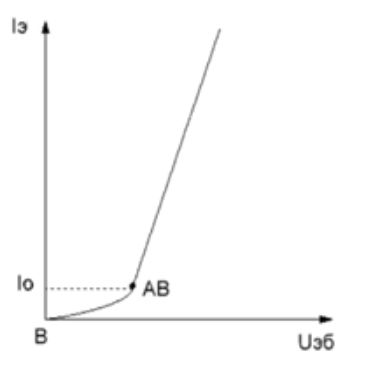
\includegraphics[width=0.7\linewidth]{photo/transistor_char}
	\caption{Входная характеристика биполярного транзистора}
	\label{fig:transistor_char}
\end{figure}

\subsection{Расчёт ВК}

Дано:

$ U_{вых. макс} = 10~В $

$ I_{н. макс} = 1.4~А, I_э \approx I_к $

$ \beta_{мин} = \dfrac{I_к}{I_б} = 100 $ (для всех транзисторов)

$ \beta $ – статический коэффициент передачи
по току транзистора в схеме с общим эмиттером.

Определим минимальное сопротивление нагрузки:

$ R_{н. мин} = \dfrac{U_{вых}}{I_{н. макс}} = \dfrac{10}{1.4} = 7.143~Ом $

Сопротивление $ R_6 $ выбираем из условия
обеспечения напряжения $ U_{вых. макс} = 10~В $
при $ I_н = I_{н. макс} $. 
В этом режиме через транзистор $ VT1 $ течёт 
минимальный ток $ I_{э_1. мин} $. 
Зададимся минимальным током $ I_{э_1. мин} = 2~мА $.
Более маленькое значение брать нельзя, потому
что транзистор теряет усилительные свойства.
При этом в цепи $ VT3 $ течёт максимальный ток:\\

$
I_{Б_3. макс} = \dfrac{I_{н. макс}}{\beta_{мин.3}} =
\dfrac{1.4}{100} = 14~мА;
I_{к3} \approx I_{э_3} = I_{н. макс}
$\\

$ I_{R_6} = I_{э_1. мин} + I_{Б_3. макс} = 2 + 14 = 16~мА $\\

\newcommand{\RomanNumeralCaps}[1]
{
	\MakeUppercase{\romannumeral #1}
}

В этом режиме из \RomanNumeralCaps{2} закона Кирхгофа:\\

$ U_{ип} = U_{R_6} + U_{ЭБ. 3} + U_{R_8} + U_{вых. макс} $\\

$ U_{ЭБ. 3} = 0.8~В; U_R \approx 0.2~В $\\

$
U_{R_6} = 
U_{ип} - U_{R_8} - U_{ЭБ. 3} - U_{вых. макс} = 
15 - 0.2 - 0.8 - 10 = 4~В
$\\

$ 
R_6 = 
\dfrac{U_{R_6}}{I_{R_6}} = 
\dfrac{4}{16 * 10^{-3}} = 
250~Ом 
$\\

Сопротивление в резисторах не более трёх значащих цифр, 
так как точность их изготовления --- 5 -- 10 \%.
Округляем значение сопротивления 
от $ 250~Ом $ (Ом) до $ 240~Ом $,
номинала из ряда E24.

Аналогичным образом определим $ R_7 $, $ R_8 $ 
из условия обеспечения напряжения 
$ -U_{вых.м} = -10~В $. 
$ I_{Н} = -I_{НМ} = -1.2~А $.
$ \beta_{мин. 3} = \beta_{мин. 4} $.\\

$ R_7 \approx R_6 = 240~Ом $\\

$ I_{R_8} \approx I_{н. макс} = 1.4~А $\\

$
R_9 = R_8 \approx 
\dfrac{U_{R_8}}{I_{н. макс}} = 
\dfrac{0.2}{1.4} = 0.143~Ом
$\\

\subsection{Максимальные мощности, рассеиваемые на элементах ВК}

Мощность рассеяния на коллекторе транзистора

$$ P_К = I_К * U_{КЭ}, $$

где: 
$ I_К $ --- ток коллектора,
$ U_{КЭ} $ --- напряжение коллектор-эммитер.\\

$
Р_{К_З. макс} \approx
Р_{К_4. макс} \approx
\dfrac{U_{ип}^2}{4 * R_{н. мин}} =
\dfrac{15^2}{4 * 7.143} =
7.875~Вт
$\\

Транзисторы $ VT1 $ и $ VT2 $
можно использовать без теплоотвода.

Определим максимальную мощность
на резисторе $ R_6 $\\
при $ U_{вых} = -U_{вых. макс} $:\\

$
U_{ип} =
U_{R_6 макс} + U_{ЭБ. 1} + U_{ЭБ. 2} - 
U_{ЭБ. 4} - U_{R_9} - U_{вых. макс}
$

$
U_{R_6 макс} =
U_{ип} + U_{ЭБ. 4} + U_{R_9} + U_{вых. макс} 
- U_{ЭБ. 1} - U_{ЭБ. 2} =
15 + 0.8 + 0.2 + 10 - 0.6 - 0.6 \approx
25~Вт
$\\

$ 
Р_{R_7 макс} \approx
P_{R_6 макс} = 
\dfrac{U_{R_6 макс}^2}{R_6} = 
\dfrac{25^2}{240} =
2.604~Вт
$\\

$
Р_{R_9 макс} \approx
Р_{R_8 макс} = 
I_{н. макс} * R_8 = 
(1.4)^2 \times 0.143 = 
0.280~Вт
$

